\setcounter{section}{3}
\setcounter{subsection}{0}

\section{Extensões do Conceito de Limite}

% ==============================================================================
% 4.1. LIMITES NO INFINITO
% ==============================================================================
\subsection{Limites no Infinito}

\begin{exercicio}[1]
Calcule:
\begin{enumerate}[label=\alph*)]
    \item $\lim\limits_{x \to +\infty} \dfrac{1}{x^2}$
    \item $\lim\limits_{x \to -\infty} \dfrac{1}{x^3}$
    \item $\lim\limits_{x \to -\infty} \left[5 + \dfrac{1}{x} + \dfrac{3}{x^2}\right]$
    \item $\lim\limits_{x \to +\infty} \left[2 - \dfrac{1}{x}\right]$
    \item $\lim\limits_{x \to +\infty} \dfrac{2x + 1}{x + 3}$
    \item $\lim\limits_{x \to -\infty} \dfrac{2x + 1}{x + 3}$
    \item $\lim\limits_{x \to -\infty} \dfrac{x^2 - 2x + 3}{3x^2 + x + 1}$
    \item $\lim\limits_{x \to +\infty} \dfrac{5x^4 - 2x + 1}{4x^4 + 3x + 2}$
    \item $\lim\limits_{x \to -\infty} \dfrac{x}{x^2 + 3x + 1}$
    \item $\lim\limits_{x \to -\infty} \dfrac{2x^3 + 1}{x^4 + 2x + 3}$
    \item $\lim\limits_{x \to +\infty} \sqrt[3]{5 + \dfrac{2}{x}}$
    \item $\lim\limits_{x \to -\infty} \sqrt[3]{\dfrac{x}{x^2 + 3}}$
    \item $\lim\limits_{x \to +\infty} \dfrac{\sqrt{x^2 + 1}}{3x + 2}$
    \item $\lim\limits_{x \to +\infty} \dfrac{\sqrt[3]{x^3 + 2x - 1}}{\sqrt{x^2 + x + 1}}$
    \item $\lim\limits_{x \to +\infty} \dfrac{\sqrt{3} + \sqrt[3]{x}}{x^2 + 3}$
    \item $\lim\limits_{x \to +\infty} \dfrac{3}{\sqrt{x}}$
    \item $\lim\limits_{x \to +\infty} \left[x - \sqrt{x^2 + 1}\right]$
    \item $\lim\limits_{x \to +\infty} \left[\sqrt{x + 1} - \sqrt{x + 3}\right]$
\end{enumerate}
\end{exercicio}

\begin{exercicio}[2]
Sejam $f$ e $g$ definidas em $[a, +\infty[$ e tais que $\lim\limits_{x \to +\infty} \dfrac{f(x)}{g(x)} = 0$, $\lim\limits_{x \to +\infty} g(x) = 0$ e $g(x) \neq 0$ para todo $x \ge a$. Calcule, caso exista, $\lim\limits_{x \to +\infty} f(x)$.
\end{exercicio}

\begin{exercicio}[3]
\begin{enumerate}[label=\alph*)]
    \item Calcule $\lim\limits_{x \to +\infty} \dfrac{x^3 + 3x - 1}{2x^3 - 6x + 1}$
    \item Mostre que existe $r > 0$ tal que
    \[
    x > r \implies \dfrac{1}{4} < \dfrac{x^3 + 3x - 1}{2x^3 - 6x + 1} < \dfrac{3}{4}
    \]
\end{enumerate}
\end{exercicio}

\begin{exercicio}[4]
\begin{enumerate}[label=\alph*)]
    \item Calcule $\lim\limits_{x \to +\infty} \dfrac{x + 3}{x^3 + 2x - 1}$
    \item Mostre que existe $r > 0$ tal que
    \[
    x > r \implies 0 < \dfrac{x + 3}{x^3 + 2x - 1} < \dfrac{1}{2}
    \]
\end{enumerate}
\end{exercicio}

\begin{exercicio}[5]
Sejam $f$ e $g$ definidas em $[a, +\infty[$ e tais que $f(x) \ge 0$ e $g(x) > 0$ para todo $x \ge a$. Suponha que $\lim\limits_{x \to +\infty} \dfrac{f(x)}{g(x)} = L$, $L > 0$. Prove que existe $r > 0$, $r > a$, tal que para todo $x > r$:
\[
\dfrac{L}{2}\,g(x) < f(x) < \dfrac{3L}{2}\,g(x).
\]
Conclua daí que se $\lim\limits_{x \to +\infty} g(x) = 0$, então $\lim\limits_{x \to +\infty} f(x) = 0$.
\end{exercicio}

\clearpage

% ==============================================================================
% 4.2. LIMITES INFINITOS
% ==============================================================================
\subsection{Limites Infinitos}

\begin{exercicio}[1]
Calcule:
\begin{enumerate}[label=\alph*)]
    \item $\lim\limits_{x \to +\infty} (x^4 - 3x + 2)$
    \item $\lim\limits_{x \to +\infty} (5 - 4x + x^2 - x^5)$
    \item $\lim\limits_{x \to -\infty} (3x^3 + 2x + 1)$
    \item $\lim\limits_{x \to +\infty} (x^3 - 2x + 3)$
    \item $\lim\limits_{x \to +\infty} \dfrac{5x^3 - 6x + 1}{6x^3 + 2}$
    \item $\lim\limits_{x \to +\infty} \dfrac{5x^3 - 6x + 1}{6x^2 + x + 3}$
    \item $\lim\limits_{x \to +\infty} \dfrac{5x^3 + 7x - 3}{x^4 - 2x + 3}$
    \item $\lim\limits_{x \to -\infty} \dfrac{2x + 3}{x + 1}$
    \item $\lim\limits_{x \to -\infty} \dfrac{x^4 - 2x + 3}{3x^4 + 7x - 1}$
    \item $\lim\limits_{x \to -\infty} \dfrac{5 - x}{3 + 2x}$
    \item $\lim\limits_{x \to +\infty} \dfrac{x + 1}{x^2 - 2}$
    \item $\lim\limits_{x \to +\infty} \dfrac{2 + x}{3 + x^2}$
\end{enumerate}
\end{exercicio}

\begin{exercicio}[2]
Prove que $\lim\limits_{x \to +\infty} \sqrt[n]{x} = +\infty$, no qual $n > 0$ é um natural.
\end{exercicio}

\begin{exercicio}[3]
Calcule:
\begin{enumerate}[label=\alph*)]
    \item $\lim\limits_{x \to +\infty} \dfrac{\sqrt{x} + 1}{x + 3}$
    \item $\lim\limits_{x \to +\infty} \dfrac{x + \sqrt[3]{x} + 3}{2x - 1}$
    \item $\lim\limits_{x \to +\infty} [2x - \sqrt{x^2 + 3}]$
    \item $\lim\limits_{x \to +\infty} (x - \sqrt[3]{3x^3 + 2})$
    \item $\lim\limits_{x \to +\infty} (x - \sqrt{x^2 + 3})$
    \item $\lim\limits_{x \to +\infty} (x - \sqrt{x + 3})$
    \item $\lim\limits_{x \to +\infty} (\sqrt{x + \sqrt{x}} - \sqrt{x - 1})$
    \item $\lim\limits_{x \to +\infty} (x - \sqrt[3]{2 + 3x^3})$
\end{enumerate}
\end{exercicio}

\begin{exercicio}[4]
Calcule:
\begin{enumerate}[label=\alph*)]
    \item $\lim\limits_{x \to 3^+} \dfrac{5}{3 - x}$
    \item $\lim\limits_{x \to 3^-} \dfrac{4}{x - 3}$
    \item $\lim\limits_{x \to \frac{1}{2}^-} \dfrac{4}{2x - 1}$
    \item $\lim\limits_{x \to 0^-} \dfrac{1}{x}$
    \item $\lim\limits_{x \to 0^+} \dfrac{2x + 1}{x}$
    \item $\lim\limits_{x \to 0^-} \dfrac{x - 3}{x^2}$
    \item $\lim\limits_{x \to 0^+} \dfrac{3}{x^2 - x}$
    \item $\lim\limits_{x \to 0^-} \dfrac{3}{x^2 - x}$
    \item $\lim\limits_{x \to \frac{1}{2}^+} \dfrac{3x + 1}{4x^2 - 1}$
    \item $\lim\limits_{x \to 1^-} \dfrac{2x + 3}{x^2 - 1}$
    \item $\lim\limits_{x \to 1^+} \dfrac{2x + 3}{x^2 - 1}$
    \item $\lim\limits_{x \to 3^+} \dfrac{x^2 - 3x}{x^2 - 6x + 9}$
    \item $\lim\limits_{x \to -1^+} \dfrac{2x + 1}{x^2 + x}$
    \item $\lim\limits_{x \to 0^+} \dfrac{2x + 1}{x^2 + x}$
    \item $\lim\limits_{x \to 1^+} \dfrac{3x - 5}{x^2 + 3x - 4}$
    \item $\lim\limits_{x \to 2^+} \dfrac{x^2 - 4}{x^2 - 4x + 4}$
    \item $\lim\limits_{x \to -1^+} \dfrac{3x^2 - 4}{1 - x^2}$
    \item $\lim\limits_{x \to 0^+} \dfrac{\sen x}{x^3 - x^2}$
\end{enumerate}
\end{exercicio}

\begin{exercicio}[5]
Dê exemplo de funções $f$ e $g$ tais que $\lim\limits_{x \to p^+} f(x) = L$, $L \neq 0$, $\lim\limits_{x \to p^+} g(x) = 0$, mas $\lim\limits_{x \to p^+} \dfrac{f(x)}{g(x)}$ não existe.
\end{exercicio}

\begin{exercicio}[6]
Dê exemplo de funções $f$ e $g$ tais que $\lim\limits_{x \to +\infty} f(x) = +\infty$, $\lim\limits_{x \to +\infty} g(x) = +\infty$ e $\lim\limits_{x \to +\infty} [f(x) - g(x)] \neq 0$.
\end{exercicio}

\begin{exercicio}[7]
Dê exemplo de funções $f$ e $g$ tais que $\lim\limits_{x \to +\infty} f(x) = +\infty$, $\lim\limits_{x \to +\infty} g(x) = +\infty$ e $\lim\limits_{x \to +\infty} \dfrac{f(x)}{g(x)} \neq 1$.
\end{exercicio}

\begin{exercicio}[8]
Seja $f(x) = ax^3 + bx^2 + cx + d$, em que $a > 0$, $b, c, d$ são reais dados. Prove que existem números reais $x_1$ e $x_2$ tais que $f(x_1) < 0$ e $f(x_2) > 0$.
\end{exercicio}

\begin{exercicio}[9]
Sejam $f$ e $g$ duas funções definidas em $]a, +\infty[$ tais que $\lim\limits_{x \to +\infty} \dfrac{f(x)}{g(x)} = +\infty$ e $g(x) > 0$ para todo $x > a$. Prove que existe $r > 0$ tal que para todo $x > r$, $f(x) > g(x)$.
\end{exercicio}

\clearpage

% ==============================================================================
% 4.3. SEQUÊNCIA E LIMITE DE SEQUÊNCIA
% ==============================================================================
\subsection{Sequência e Limite de Sequência}

\begin{exercicio}[1]
Calcule:
\begin{enumerate}[label=\alph*)]
    \item $\lim\limits_{n \to +\infty} \dfrac{2n - 3}{n + 1}$
    \item $\lim\limits_{n \to +\infty} n^2 + 3$
    \item $\lim\limits_{n \to +\infty} \dfrac{n + 1}{n}$
    \item $\lim\limits_{n \to +\infty} \dfrac{n^2 + 2}{2n^3 + n - 1}$
    \item $\lim\limits_{n \to +\infty} \left[\dfrac{(-1)^n}{n} + 2\right]$
    \item $\lim\limits_{n \to +\infty} \left[\dfrac{2}{n} + \left(\dfrac{3}{5}\right)^{\!n}\right]$
    \item $\lim\limits_{n \to +\infty} \dfrac{1 + 5^n}{2 + 3^n}$
    \item $\lim\limits_{n \to +\infty} \sum_{k = 0}^{n} \left(\dfrac{1}{3}\right)^{\!k}$
    \item $\lim\limits_{n \to +\infty} \sum_{k = 0}^{n} t^k$ no qual $0 < t < 1$
\end{enumerate}
\end{exercicio}

\begin{exercicio}[2]
Supondo $0 < a < 1$, mostre que:
\[
\lim_{n \to +\infty} \sum_{k = 1}^{n} a^k = \dfrac{a}{1 - a}.
\]
\end{exercicio}

\begin{exercicio}[3]
Calcule $\lim\limits_{n \to +\infty} \left(1 + \dfrac{1}{2} + \dfrac{1}{3} + \dots + \dfrac{1}{n}\right)$.\\
(\textit{Sugestão:} $\dfrac{1}{2^k} + \dfrac{1}{2^k + 1} + \dots + \dfrac{1}{2^{k+1} - 1} > \dfrac{1}{2}$ para $k \ge 0$.)
\end{exercicio}

\begin{exercicio}[4]
Seja $f(x) = x$, $x \in [0, 1]$. Considere a sequência de termo geral:
\[
S_n = f\!\left(\dfrac{1}{n}\right)\dfrac{1}{n} + f\!\left(\dfrac{2}{n}\right)\dfrac{1}{n} + f\!\left(\dfrac{3}{n}\right)\dfrac{1}{n} + \dots + f\!\left(\dfrac{n - 1}{n}\right)\dfrac{1}{n} + f(1)\dfrac{1}{n}.
\]
\begin{enumerate}[label=\alph*)]
    \item Calcule $S_3$. Observe que, geometricamente, $S_3$ pode ser interpretado como a soma das áreas dos retângulos hachurados.

\begin{center}
\begin{tikzpicture}[scale=3.5, >=latex]
    \draw[->, thick] (-0.15, 0) -- (1.3, 0) node[below] {$x$};
    \draw[->, thick] (0, -0.15) -- (0, 1.25) node[left] {$y$};
    \node[below left] at (0, 0) {$0$};

    \draw[thick, fill=gray!25] (0, 0) rectangle (1/3, 1/3);
    \draw[thick, fill=gray!25] (1/3, 0) rectangle (2/3, 2/3);
    \draw[thick, fill=gray!25] (2/3, 0) rectangle (1, 1);

    \draw[ultra thick, blue!60!black] (0, 0) -- (1, 1);

    \draw (1/3, 0.02) -- (1/3, -0.02) node[below=3pt] {$\dfrac{1}{3}$};
    \draw (2/3, 0.02) -- (2/3, -0.02) node[below=3pt] {$\dfrac{2}{3}$};
    \draw (1, 0.02) -- (1, -0.02) node[below=3pt] {$1$};

    \draw[dashed] (0, 1) -- (1, 1);
    \draw (0.02, 1) -- (-0.02, 1) node[left] {$1$};
\end{tikzpicture}
\end{center}

    \item Calcule $\lim\limits_{n \to +\infty} S_n$. (Pensando geometricamente, qual o valor esperado para o limite?)
\end{enumerate}
\end{exercicio}

\begin{exercicio}[5]
Calcule $\lim\limits_{n \to +\infty} \dfrac{1}{n^3}\sum\limits_{k=1}^n k^2$.\\
(\textit{Sugestão:} Verifique que $1^2 + 2^2 + 3^2 + \dots + n^2 = \dfrac{1}{6}n(n + 1)(2n + 1)$. Veja Seção 17.2.)
\end{exercicio}

\begin{exercicio}[6]
Seja $f(x) = x^2$, $x \in [0, 1]$. Considere as sequências:
\[
s_n = f(0)\dfrac{1}{n} + f\!\left(\dfrac{1}{n}\right)\dfrac{1}{n} + f\!\left(\dfrac{2}{n}\right)\dfrac{1}{n} + \dots + f\!\left(\dfrac{n - 1}{n}\right)\dfrac{1}{n}
\]
e
\[
S_n = f\!\left(\dfrac{1}{n}\right)\dfrac{1}{n} + f\!\left(\dfrac{2}{n}\right)\dfrac{1}{n} + \dots + f\!\left(\dfrac{n - 1}{n}\right)\dfrac{1}{n} + f(1)\dfrac{1}{n}.
\]
Calcule:
\begin{enumerate}[label=\alph*)]
    \item $\lim\limits_{n \to +\infty} S_n$
    \item $\lim\limits_{n \to +\infty} s_n$
\end{enumerate}
(Interprete geometricamente tais limites.) (\textit{Sugestão:} Utilize o Exercício 5.)
\end{exercicio}

\begin{exercicio}[7]
Uma partícula desloca-se sobre o eixo $0x$ com aceleração constante $a$, $a > 0$. Suponha que no instante $t = 0$ a velocidade seja zero. A velocidade no instante $t$ é, então, dada por $v(t) = at$. Divida o intervalo de tempo $[0, T]$ em $n$ intervalos de amplitudes iguais a $\dfrac{T}{n}$:

\begin{center}
\begin{tikzpicture}[scale=1.1, >=latex]
    \draw[thick] (0, 0) -- (7.5, 0);
    
    \draw (0, 0.15) -- (0, -0.15) node[below=3pt] {$0$};
    \draw (1.2, 0.15) -- (1.2, -0.15) node[below=3pt] {$\dfrac{T}{n}$};
    \draw (2.4, 0.15) -- (2.4, -0.15) node[below=3pt] {$\dfrac{2T}{n}$};
    \draw (3.6, 0.15) -- (3.6, -0.15) node[below=3pt] {$\dfrac{3T}{n}$};
    
    \node at (4.8, 0.2) {$\dots$};
    
    \draw (5.7, 0.15) -- (5.7, -0.15) node[below=3pt] {$\dfrac{(n-1)T}{n}$};
    \draw (7.2, 0.15) -- (7.2, -0.15) node[below=3pt] {$T$};
\end{tikzpicture}
\end{center}

No instante $\dfrac{T}{n}$ a velocidade será $\dfrac{aT}{n}$, no instante $\dfrac{2T}{n}$, será $\dfrac{2aT}{n}$, etc. Supondo $n$ suficientemente grande, o espaço percorrido entre os instantes $\dfrac{T}{n}$ e $\dfrac{2T}{n}$ será aproximadamente $\dfrac{aT}{n}\cdot\dfrac{T}{n}$ (por quê?); entre os instantes $\dfrac{2T}{n}$ e $\dfrac{3T}{n}$ o espaço percorrido será aproximadamente $\dfrac{2aT}{n}\cdot\dfrac{T}{n}$, etc.
\begin{enumerate}[label=\alph*)]
    \item Calcule $\lim\limits_{n \to +\infty} \left[\dfrac{aT}{n}\cdot\dfrac{T}{n} + \dfrac{2aT}{n}\cdot\dfrac{T}{n} + \dots + \dfrac{(n - 1)aT}{n}\cdot\dfrac{T}{n}\right]$.
    \item Interprete cinemática e geometricamente o limite acima.
\end{enumerate}
\end{exercicio}

\begin{exercicio}[8]
Suponha que a sequência de termo geral $a_n$, $n$ natural, seja crescente (isto é, quaisquer que sejam os naturais $n$ e $m$, $n < m \implies a_n \le a_m$) e que exista $M$ real tal que $a_n \le M$ para todo natural $n$. Prove que $\lim\limits_{n \to +\infty} a_n$ existe e que $\lim\limits_{n \to +\infty} a_n = \sup[a_n \mid n \in \N]$. (Veja Seção A.4.)
\end{exercicio}

\begin{exercicio}[9]
Considere a sequência de termo geral:
\[
a_n = 1 + \dfrac{1}{2^2} + \dfrac{1}{3^2} + \dots + \dfrac{1}{n^2}.
\]
\begin{enumerate}[label=\alph*)]
    \item Prove que $a_n$ é crescente.
    \item Prove que para todo natural $n \ge 1$:
    \[
    1 + \dfrac{1}{2^2} + \dfrac{1}{3^2} + \dots + \dfrac{1}{n^2} < 2.
    \]
    \item Prove que $\lim\limits_{n \to +\infty} \left(1 + \dfrac{1}{2^2} + \dfrac{1}{3^2} + \dots + \dfrac{1}{n^2}\right)$ existe e que é menor que $2$. (Compare com o Exercício 3.)
\end{enumerate}
(\textit{Sugestão para (b):} Verifique que $\dfrac{1}{(2^n)^2} + \dfrac{1}{(2^n + 1)^2} + \dots + \dfrac{1}{(2^{n+1} - 1)^2} \le \dfrac{1}{2^n}$.)
\end{exercicio}

\clearpage

% ==============================================================================
% 4.4. LIMITE DE FUNÇÃO E SEQUÊNCIAS
% ==============================================================================
\subsection{Limite de Função e Sequências}

\begin{exercicio}[1]
Seja $f(x) = \begin{cases} x & \text{se } x \in \Q \\ -x & \text{se } x \notin \Q \end{cases}$.
\begin{enumerate}[label=\alph*)]
    \item Calcule $\lim\limits_{x \to 0} f(x)$.
    \item Mostre que, para todo $p \neq 0$, $\lim\limits_{x \to p} f(x)$ não existe.
\end{enumerate}
\end{exercicio}

\begin{exercicio}[2]
Seja a sequência de termo geral $a_n$, com $a_n > 0$ para todo natural $n$. Sabe-se que $\lim\limits_{n \to +\infty} a_n = a$, $a$ real, e que $a_{n+1} = \dfrac{1}{1 + a_n}$ para todo $n$. Calcule $a$.
\end{exercicio}

\begin{exercicio}[3]
Sejam $f$ uma função, $p$ um número real e suponha que existam duas sequências $a_n$ e $b_n$ convergindo a $p$, com $a_n$ e $b_n$ pertencentes a $D_f$ para todo $n$, tais que:
\[
\lim_{n \to +\infty} f(a_n) = L \quad\text{e}\quad \lim_{n \to +\infty} f(b_n) = L.
\]
Podemos, então, afirmar que $\lim\limits_{x \to p} f(x) = L$? Por quê?
\end{exercicio}

\begin{exercicio}[4]
Sabe-se que a sequência $a_1 = \sqrt{2}$, $a_2 = \sqrt{2\sqrt{2}}$, $a_3 = \sqrt{2\sqrt{2\sqrt{2}}}$, \dots, é convergente. Calcule $\lim\limits_{n \to +\infty} a_n$.
\end{exercicio}

\begin{exercicio}[5]
Sabe-se que a sequência $\sqrt{2}$, $\sqrt{2 + \sqrt{2}}$, $\sqrt{2 + \sqrt{2 + \sqrt{2}}}$, \dots, é convergente. Calcule seu limite.
\end{exercicio}

\begin{exercicio}[6]
Prove que $\lim\limits_{x \to 0} \sen\dfrac{1}{x}$ não existe.
\end{exercicio}

\clearpage

% ==============================================================================
% 4.5. O NÚMERO e
% ==============================================================================
\subsection{O Número $e$}
\textit{Esta subseção não possui exercícios.}
